\documentclass[a4paper,11pt]{article}
\usepackage[english]{babel}
\usepackage[utf8]{inputenc}
\usepackage{amsmath,amsfonts,amsthm,amssymb,mathtools,dsfont}
\usepackage{tikz}

\renewcommand{\to}[1]{\text{\boldmath $#1$}} % Bold, cursive
\newcommand{\ts}[1]{\text{\boldmath $\mathrm{#1}$}} % Bold, straigt
\newcommand{\td}[1]{\text{\boldmath $\mathcal{#1}$}} % Bold, 
\newcommand{\tf}[1]{\text{\boldmath $\mathsf{#1}$}} % Bold, sans-serif
\newcommand{\uv}[1]{\mathds{#1}}
\newcommand{\um}[1]{\mathds{#1}}
\newcommand{\intd}[1]{\mathrm{d}#1}
\newcommand{\pderiv}[2]{\frac{\partial#1}{\partial#2}}
\newcommand{\dderiv}[2]{\frac{\mathrm{d}#1}{\mathrm{d}#2}}
\newcommand{\norm}[1]{\left\lVert{#1}\right\rVert}
\newcommand{\T}{\mathrm{T}}
\newcommand{\defeq}{:=}
\newcommand{\element}{\mathrm{e}}
\newcommand{\linear}{\mathrm{lin}}
\DeclareMathOperator{\diff}{D}

\begin{document}
\section{Surface tension in FEA}
This document derives expressions necessary to calculate the load vector in FE analysis for isotropic surface tension. First rewriting the curvature in order to avoid the second derivative.
\begin{align}
 \int_\Omega 2 H \to w\cdot \to n\intd A = \int_{\partial\Omega} \to w\cdot\to m\intd S - \int_\Omega \to \nabla_s \cdot \to w \intd A
\end{align}

\section{Extruded 2D}

\begin{figure}[htpb]
 \centering
 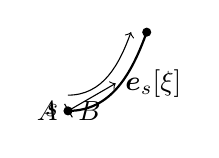
\begin{tikzpicture}
  \draw[thick] (0,0) to[out=0,in=250] (1,1) coordinate[near start] (m) node[at start,left] {$A$} node[at end,right] {$B$};
  \draw[->] (0,0.2) to[out=0,in=250] (0.8,1) node[at end,left] {$s$};
  \draw[|->] (m) -- +(30:0.7) node[at end,right] {$\to e_s[\xi]$};
  \draw[fill,black] (0,0) circle (0.05) (1,1) circle (0.05);
 \end{tikzpicture}
 \caption{Geometry and coordinate system for 2D (and axisymmetric)}
\end{figure}

\begin{align}
 \to x &= \sum_i N_i[\xi]\to x_i
\end{align}

\begin{gather}
 \dderiv{s}{\xi} = \norm{\dderiv{\to x}{\xi}} = J\\
 \to e_s = \dderiv{\to x}{\xi} J^{-1}\\
 \intd A = t \intd s = t J \intd \xi\\
 \to \nabla_s = \pderiv{}{s}\to e_s = \pderiv{}{\xi}\to e_s J
\end{gather}

After applying the divergence theorem to the curvature integral, we obtain
\begin{align}
  &\int_\Omega\to \nabla_s\cdot\to w\intd A\\
 =&\int_A^B\dderiv{\to w}{s}\cdot\to e_s t \intd s\\
 =&t \int_a^b \dderiv{\to w}{\xi}\cdot \to e_s \intd\xi\\
\end{align}
and its tangent, calculated easily with the following derivations
\begin{gather}
 \pderiv{\to x'}{\to x_i} = N_i' \ts I\\
 \pderiv{J}{\to x_i} = J^{-1} \to x'\cdot \pderiv{\to x'}{\to x_i} = J^{-1} N_i' \to x'
\end{gather}
to obtain
\begin{align}
 \int_\Omega\to \nabla_s\cdot\to w\intd A \otimes \pderiv{}{\to x_i}
 =&t \int_a^b \left(\dderiv{\to w}{\xi}\cdot \to e_s\right)\otimes \pderiv{}{\to x_i}  \intd\xi\\
 =&t \int_a^b \dderiv{\to w}{\xi}\cdot \pderiv{\to e_s}{\to x_i} \intd\xi\\
 =&t \int_a^b \dderiv{\to w}{\xi}\cdot \left(\pderiv{\to x'}{\to x_i}J^{-1}-\to x'\otimes\pderiv{J}{\to x_i}J^{-2}\right) \intd\xi\\
 =&t \int_a^b \dderiv{\to w}{\xi}\cdot \left(\ts I-\to x'\otimes\to x' J^{-2}\right)N_i' J^{-1} \intd\xi
\end{align}

The boundary term is trivial
\begin{align}
 &\int_{\partial\Omega} \to w\cdot \to m\intd S = \to w \cdot\to m t = - \to w \cdot \to e_s t
\end{align}
and its tangent
\begin{align}
 \int_{\partial\Omega} \to w\cdot \to m\intd S\otimes \pderiv{}{\to x_i} &= -t(\to w \cdot \to e_s)\otimes \pderiv{}{\to x_i}\\
 &= -t \to w\cdot\pderiv{\to e_s}{\to x_i}\\
 &= -t \to w\cdot \left(\ts I-\to x'\otimes\to x' J^{-2}\right)N_i' J^{-1}
\end{align}
for a boundary located at $\to x_1$.

The load vector for a load along one edge and the special case of linear edges becomes
\begin{gather}
 \to w = \um{N}\cdot\um{C} = \begin{bmatrix}N_1 & 0 & \cdots\\ 0 & N_1 & \cdots \end{bmatrix}\cdot \um{C}\\
 \uv F^\element = \gamma t \int_a^b \dderiv{{\um N^\element}^\T}{\xi}\cdot \to e_s \intd\xi\\
 \um K^\element = 
\end{gather}
\begin{gather}
 \uv F^\element = \gamma t \begin{bmatrix}m_x\\m_y\end{bmatrix} = - \gamma t \begin{bmatrix}e_{s,x}\\e_{s,y}\end{bmatrix}
 \um K^\element = 
\end{gather}
and the special case of linear elements
\begin{gather}
 \uv F^\element_\linear = \gamma t L^{-1} \begin{bmatrix}x_2-x_1\\y_2-y_1\\x_1-x_2\\y_1-y_2\end{bmatrix}\\
 \um K^\element_\linear = \gamma t L^{-1}\left(
	\begin{bmatrix}-1&0&1&0\\0&-1&0&1\\1&0&-1&0\\0&1&0&-1\end{bmatrix}+
	L^{-2}\begin{bmatrix}x_2-x_1\\y_2-y_1\\x_1-x_2\\y_1-y_2\end{bmatrix}\cdot\begin{bmatrix}x_2-x_1\\y_2-y_1\\x_1-x_2\\y_1-y_2\end{bmatrix}^\T
  \right)
\end{gather}
and for the boundary
\begin{gather}
 \uv F^\element_\linear = \gamma t L^{-1} \begin{bmatrix}x_1-x_2\\y_1-y_2\end{bmatrix}\\
 \um K^\element_\linear = \gamma t L^{-1} \left(\begin{bmatrix}1&0&-1&0\\0&1&0&-1\end{bmatrix} + L^{-2} \begin{bmatrix}x_2-x_1\\y_2-y_1\end{bmatrix}\cdot\begin{bmatrix}x_2-x_1\\y_2-y_1\\x_1-x_2\\y_2-y_1\end{bmatrix}^\T\right)\\
\end{gather}

\section{Axisymmetric}
This part was more complicated than initially estimated.
I have consistently decomposed variables into $\ts Q$ to make this managable and also analytically calculating the integral over $\theta$.

With cylindrical coordinates $\to r = r\to e_r + z \to e_z$.
\begin{align}
 \to r &= \sum_i N_i[\xi]\to r_i\\
 x &= \cos[\theta] r\\
 y &= \sin[\theta] r\\
 z &= z\\
 \ts Q &= \begin{bmatrix}\cos[\theta] & 0\\ \sin[\theta] & 0\\ 0 & 1\end{bmatrix}\\
 \to x &= \ts Q[\theta] \cdot \to r[\xi]\\
 \to w &= \ts Q[\theta] \cdot \to v[\xi]
\end{align}

Since we have a convenient orthogonality, we can treat $\xi$ and $\theta$ seperarely.
\begin{align}
 J_\xi &= \norm{\pderiv{\to x}{\xi}} = \norm{\ts Q \cdot \to r'} = \norm{\to r'}\\
 J_\theta &= \norm{\pderiv{\to x}{\theta}} = \norm{\ts Q' \cdot \to r} = r \\
 \intd A &= J_\xi J_\theta \intd \xi \intd \theta \\
 \to\nabla_s &= J_\xi^{-2} \pderiv{\to x}{\xi}\pderiv{}{\xi} + J_\theta^{-2} \pderiv{\to x}{\theta}\pderiv{}{\theta}
\end{align}

\begin{align}
 &\int_\Omega\to \nabla_s\cdot\to w\intd A\\
=&\int_a^b\int_0^{2\pi}\left( J_\xi^{-2} \pderiv{\to x}{\xi}\cdot\pderiv{\to w}{\xi} +
                              J_\theta^{-2} \pderiv{\to x}{\theta}\cdot\pderiv{\to w}{\theta}
  \right) J_\xi J_\theta \intd \theta \intd \xi\\
=&\int_a^b\int_0^{2\pi}\left(
	  J_\xi^{-2} (\ts Q^\T\cdot\ts Q):(\to r'\otimes \to v') +
	  J_\theta^{-2} ({\ts Q'}^\T\cdot\ts Q'):(\to r\otimes\to v)
  \right) J_\xi J_\theta \intd \theta \intd \xi\\
=&\int_a^b\int_0^{2\pi}\left(
	  J_\xi^{-2} \ts I :(\to r'\otimes \to v') +
	  J_\theta^{-2} \begin{bmatrix}1&0\\0&0\end{bmatrix}:(\to r \otimes \to v)
  \right) J_\xi J_\theta \intd \theta \intd \xi\\
=&2\pi\int_a^b\left(
	  \norm{\to r'}^{-1} r \to r' \cdot \to v' +
	  \norm{\to r'} v_1
  \right) \intd \xi
\end{align}

The boundary term is computed as
\begin{align}
 \to m &= \ts Q\cdot \to t\\
 &\int_{\partial\Omega} \to w\cdot\to m\intd S\\
=&\int_0^{2\pi} (\ts Q^\T\cdot \ts Q):(\to v\cdot\to t) r \intd \theta\\
=& 2\pi r \to v \cdot \to t
\end{align}

The load vector for a load along one edge and the special case of linear edges becomes
\begin{gather}
 \to v = \um{N}\cdot\um{C} = \begin{bmatrix}N_1 & 0 & \cdots\\ 0 & N_1 & \cdots \end{bmatrix}\cdot \um{C}\\
 \um F^\element = 2\pi \gamma \int_a^b \left(\norm{\to r'}^{-1}r\to r'\cdot{\um N^\element}'^\T + \norm{\to r'}{\um N^\element}^\T\cdot\begin{bmatrix}1&0\end{bmatrix}\right) \intd\xi\\
 \um F^\element = 2\pi \gamma r \begin{bmatrix}t_1\\t_2\end{bmatrix}
\end{gather}
and the special case of linear elements
\begin{gather}
 \um F^\element_\linear = \pi \gamma \left(\frac{r_1+r_2}{L}\begin{bmatrix}r_1-r_2\\z_1-z_2\\r_2-r_1\\z_2-z_1\end{bmatrix} + L\begin{bmatrix}1\\0\\1\\0\end{bmatrix}\right)
\end{gather}

\section{General 3D}

Introducing another parameter $\zeta$ in order to obtain a nice mapping.
\begin{align}
 \to x[\xi,\eta,\zeta] = (1-\zeta)\sum_i N_i[\xi,\eta]\to x_i
\end{align}

\begin{gather}
 J \defeq \norm{\pderiv{\to x}{\xi} \times  \pderiv{\to x}{\eta}}\\
 \to n = \pderiv{\to x}{\xi} \times \pderiv{\to x}{\eta} J^{-1}\\
 %\to \nabla = \pderiv{}{x}\to e_x + \pderiv{}{y}\to e_y + \pderiv{}{z}\to e_z\\
 \begin{bmatrix}\intd x\\ \intd y\\ \intd z\end{bmatrix} =
  \underbrace{\begin{bmatrix}\pderiv{x}{\xi} & \pderiv{x}{\eta} & \pderiv{x}{\zeta}\\
	  \pderiv{y}{\xi} & \pderiv{y}{\eta} & \pderiv{y}{\zeta}\\
	  \pderiv{z}{\xi} & \pderiv{z}{\eta} & \pderiv{z}{\zeta} \end{bmatrix}}_{\ts J}
  \cdot \begin{bmatrix}\intd \xi \\ \intd \eta \\ \intd \zeta\end{bmatrix}\\
 \to\nabla = \ts J^{-\T}\cdot\to\nabla_\xi\\
 \intd A = J \intd \xi \intd \eta 
\end{gather}

%If i do some handwaving instead, similar to Perić (perhaps this is only possible when i have axisymmetry, and i don't necessarily have orthogonality now?)

%\begin{align}
% \to \nabla_s &= \pderiv{}{s}\to e_s + \pderiv{}{t}\to e_t\\
% \begin{bmatrix}\intd s\\ \intd t\end{bmatrix} &= \begin{bmatrix}\pderiv{s}{\xi} & \pderiv{s}{\eta} \\ \pderiv{t}{\xi} & \pderiv{t}{\eta}\end{bmatrix} \cdot \begin{bmatrix}\intd \xi\\ \intd \eta\end{bmatrix}\\
% \intd s_i &= \pderiv{s_i}{\xi_j} \intd \xi_j\\
% \intd A &= \det[\ts J] \intd \xi \intd \eta
%\end{align}

%\begin{gather}
% \intd A = \intd s \intd t = \begin{vmatrix}\pderiv{s}{\xi} & \pderiv{s}{\eta}\\ \pderiv{t}{\xi} & \pderiv{t}{\eta}\end{vmatrix}\intd \xi \intd \eta = J \intd \xi \intd \eta
%\end{gather}

and we obtain
\begin{align}
 &\iint_\Omega\to \nabla_s\cdot\to w\intd A\\
=&\iint_\omega(\ts I-\to n\otimes\to n):(\to w\otimes \ts J^{-\T}\cdot\to\nabla_\xi)J\intd\xi\intd\eta\big|_{\zeta=1}\\
=&\iint_\omega(\ts I-\to n\otimes\to n):\left((\to w\otimes\to\nabla_\xi) \cdot\ts J^{-1}\right)J\intd\xi\intd\eta\big|_{\zeta=0}\\
=&\iint_\omega((\ts I-\to n\otimes\to n)\cdot\to J^{-\T}):(\to w\otimes\to\nabla_\xi)J\intd\xi\intd\eta\big|_{\zeta=0}
\end{align}

And given an edge along $\xi$;
\begin{align}
 &\int_{\partial\Omega}\to w\cdot\to m\intd S\\
=&\int_{\partial\omega}\to w\cdot\to m\norm{\pderiv{\to x}{\xi}}\intd \xi\\
 \hat{\to n} &= \to e_\xi \times \to e_\eta\\
 \hat{\to m} &= \to e_\xi \times \hat{\to n} = \to e_\xi\times (\to e_\xi \times \to e_\eta)\\
 \to m &= \hat{\to m}\norm{\to m}^{-1}
\end{align}


\section{General 3D alternative method}
\begin{align}
 \to x[\xi,\eta] = \sum_i N_i[\xi,\eta]\to x_i
\end{align}

\begin{gather}
 J \defeq \norm{\pderiv{\to x}{\xi} \times  \pderiv{\to x}{\eta}}\\
 \to n = \pderiv{\to x}{\xi} \times \pderiv{\to x}{\eta} J^{-1}\\
 \to e_s = \pderiv{\to x}{\xi}\norm{\pderiv{\to x}{\xi}}^{-1}\\
 \to e_t = -\to e_s\times \to n\\
 \begin{bmatrix}\intd x\\ \intd y\\ \intd z\end{bmatrix} =
  \underbrace{\begin{bmatrix}\pderiv{\to x}{\xi} & \pderiv{\to x}{\eta}
  \end{bmatrix}}_{\ts J''}
  \cdot \begin{bmatrix}\intd \xi \\ \intd \eta\end{bmatrix}\\
 \begin{bmatrix}\intd s\\ \intd t\end{bmatrix} =
  \underbrace{\begin{bmatrix} \to e_s^\T \\ \to e_t^\T
  \end{bmatrix}}_{\ts J'}
  \cdot \begin{bmatrix}\intd x \\ \intd y \\ \intd z\end{bmatrix}\\
 \intd A = J \intd \xi \intd \eta
\end{gather}

\begin{align}
 \to\nabla_s\cdot\to w &= \to\nabla_{st}\cdot\to w_{st} \\
 &= (\to w_{st}\otimes\to\nabla_{st}):\ts I \\
 &= \left(((\ts J'\cdot \to w) \otimes \to\nabla_{\xi\eta})\cdot \left(\ts J'\cdot\ts J''\right)^{-1}\right): \ts I\\
 &= \left((\to w\cdot (\ts J'^\T \otimes \to\nabla_{\xi\eta}) +\ts J'\cdot(\to w\otimes\to\nabla_{\xi\eta}) )\cdot \left(\ts J'\cdot\ts J''\right)^{-1}\right): \ts I
\end{align}
The gradient $\ts J'^\T \otimes\to\nabla_{\xi\eta}$ is bothersome.
\begin{align}
 \to e_s \otimes \to\nabla_{\xi\eta} = \text{ugh...}
\end{align}

Considering the special case of linear surfaces;
\begin{align}
  \to\nabla_s\cdot\to w &= \left(\ts J'\cdot(\to w\otimes\to\nabla_{\xi\eta})\cdot \left(\ts J'\cdot\ts J''\right)^{-1}\right): \ts I
\end{align}

\begin{align}
 &\iint_\Omega\to \nabla_s\cdot\to w\intd A\\
=&\iint_\omega \ts I:\left(\ts J'\cdot(\to w\otimes\to\nabla_{\xi\eta})\cdot \left(\ts J'\cdot\ts J''\right)^{-1}\right)J\intd\xi\intd\eta
\end{align}

\end{document}
